\chapter{Grundlagen} \label{cha:grundlagen}
Die vorliegende Schrift ist grundsätzlich als Forschung- und Entwicklungsarbeit des automatisierten Fahrens in der Automobilbranche anzusiedeln. Es werden zunächst nötige Begrifflichkeiten definiert und in aller Kürze der industrielle Entwicklungsfortschritt hin zum vollautomatisierten Fahren vorgestellt und damit ein Projektbezug geschaffen.\\
Der zentrale Teil der Arbeit liegt in dem Aufbau einer Datenbuskommunikation mit dem Demonstratorfahrzeug zur strukturierten Auswertung der Fahrzeugzustandsdaten. Daher werden zudem einige wichtige Informationen zu Bussystemen und der Datenkommunikation im Fahrzeug vorgestellt. Es gilt zu erwähnen, dass dieser Teilabschnitt aufgrund der thematischen Schnittmenge teilweise aus der vorangegangenen Bachelorarbeit \cite{Kary.12.09.2016} des Verfassers übernommen wurde.

\section{Autonomes Fahren} \label{sec:AutonomesFahren}
% Unterschied automatisiertes/autonomes Fahren
Fast alle aktuellen am Markt befindlichen Fahrzeuge bieten eine Vielzahl verschiedener Fahrerassistenzsysteme. Dies wurde in den vergangen Jahren sowohl durch stetig steigenden Kundenforderungen nach mehr Sicherheit und einem erhöhten Fahrkomfort, als auch durch den Innovationsdrang der gesamten Automobilindustrie möglich. Gängige Fahrerassistenzsysteme sorgen dabei in kritischen Situationen für eine erhöhte Fahrstabilität, halten automatisch Abstand zum vorausfahrenden Fahrzeug oder unterstützen den Fahrer bei Parkmanövern. Durch den kontinuierlichen Einzug innovativer Sensorik, leistungsstarker Steuergeräte und einer stetigen Optimierung der Datenverarbeitung ist hier jedoch noch längst nicht Schluss. Verschiedenen Einschätzungen zufolge, wird das autonome Fahren in 10 bis 20 Jahren  marktreif sein \cite{Winner.2015}. Autonomes Fahren könnte einen Umbruch im individuellen und gesellschaftlichen Umgang mit dem Automobil nach sich ziehen und damit auch Einfluss nehmen auf Verkehr, Mobilität oder Raumstrukturen. Auf dem Weg dahin, gibt es jedoch zunächst etliche technische, rechtliche und ethische Herausforderungen auf nationaler und internationaler Ebene zu bewältigen. In den Medien stößt man immer wieder auf unterschiedliche Meinungen und Erklärungen im Zusammenhang mit dem automatischen, automatisierten oder autonomen Fahren. Daher gilt es, diese Begrifflichkeiten zunächst klar zu definieren und voneinander abzugrenzen. 

\subsection{Autonomiestufen} \label{subsec:Autonomiestufen}% 5-Stufen des autonomen Fahrens
Das autonome Fahren wird umgänglich mit einem Autopiloten assoziiert, der sämtliche Fahrmanöver auf Stabilisierungs-, Bahnführungs- und Navigationsebene ohne ein menschliches Eingreifen durchführen kann. Im konkreten Zusammenhang mit mobilen Robotern spricht man eher von einer Autonomie, wenn sich ein Roboter in seiner Umgebung selbstständig bewegen und agieren kann. Der Roboter agiert jedoch nur so lange autonom, wie seine Energieversorgung dies zulässt.\\
Um Missverständnisse zu vermeiden und einheitliche Entwicklungsziele auf internationaler Ebene setzen zu können, hat die \emph{Society of Automotive Engineers} \acs{SAE} International in der Norm \emph{SAE J3016} \cite{SAEInternational.15.06.2018} sechs Stufen definiert, um Begriffe für straßengebundene Kraftfahrzeuge mit Systemen zum autonomen Fahren einheitlich zu beschreiben. Die sechs Autonomiestufen der Norm sind in Tabelle \ref{tab:AutonomiestufenSAE} gelistet. Diese Interpretation der Klassifizierung beschreibt, welche Aufgaben das System selbst wahrnimmt und welche Anforderungen dabei an den Fahrer gestellt werden.

\begin{table}[!htb]
	\centering
	\caption{Sechs Stufen der Autonomie für straßengebundene Kraftfahrzeuge nach \emph{SAE\,J3016} \cite{VerbandderAutomibilindustriee.V..2015}.}
	\renewcommand{\arraystretch}{1.3}
	\begin{tabular}{l  l | p{8.5cm}}
		\toprule
		Stufe & Bezeichnung & Definition \\ 
		\midrule
		0 & keine Automation & Fahrer führt dauerhaft Längs- \emph{und} Querführung aus. Kein eingreifendes Fahrzeugsystem aktiv.\\
		1 & Assistenzsysteme & Fahrer führt dauerhaft Längs- \emph{oder} Querführung aus. System übernimmt die jeweils andere Funktion.\\
		2 & Teilautomatisierung & Fahrer \emph{muss} das System dauerhaft überwachen. System übernimmt Längs- \emph{und} Querführung in einem spezifischen Anwendungsfall\footnotemark.\\
		3 & Bedingte Automatisierung & Fahrer \emph{muss} das System \emph{nicht} mehr \emph{dauerhaft} überwachen. Fahrer muss potentiell in der Lage sein, zu übernehmen. System übernimmt Längs- \emph{und} Querführung in einem spezifischen Anwendungsfall. Systemgrenzen werden alle erkannt. Ausreichende Zeitreserve zur Übernahme.\\
		4 & Hochautomatisierung & Kein Fahrer erforderlich im spezifischen Anwendungsfall. System kann im spezifischen Anwendungsfall \emph{alle Situationen} automatisch bewältigen.\\
		5 & Vollautomatisierung & Von \emph{Start} bis \emph{Ziel} ist kein Fahrer erforderlich. System übernimmt Fahraufgabe \emph{vollumfänglich} in allen Situation.\\
		\bottomrule
	\end{tabular}
	\label{tab:AutonomiestufenSAE}
\end{table}
\footnotetext{Anwendungsfälle beinhalten Straßentypen, Geschwindigkeitsbereiche und Umfeldbedingungen.}

Ein Wechsel der Autonomiestufe tritt bedingt durch die Ausweitung der Assistenzfunktionen und deren Systemintegration auf. Es gilt zu beachten, dass nach dieser Definition bis zur Autonomiestufe vier ein Fahrzeugführer jederzeit in der Lage sein muss, die Fahraufgabe vollständig und nahtlos zu übernehmen.\\
Rein passive Systeme wie Spurverlassenswarner oder Totwinkelwarner sind bereits seit einigen Jahren verfügbar und bilden in Autonomiestufe 0 den Einstieg in die Entwicklung hin zu vollautomatisierten Fahrzeugsystemen. Als Vertreter der Autonomiestufe 1 sind Systeme wie adaptive Geschwindigkeitsregelung oder Spurhalteassistenten zu nennen. Diese Systeme übernehmen zeitweise eine Längs- oder Querführung und sind heute flächendeckend in der Serie zu finden. Eine Kombination aus Längs- und Querführung ist Basis für die Autonomiestufe 2. Als Beispiel hierfür ist ein Stauassistent zu nennen, der bei geringen Geschwindigkeiten die Längs- und Querführung des Fahrzeuges übernimmt. Aufgrund der aufwändigen Kombination unterschiedlicher Sensorsysteme und der daraus resultierenden Sensordatenfusion sind solche Funktionen aktuell lediglich in hochklassigen Fahrzeugen zu finden. In der Autonomiestufe 3 sind solche Systeme für höhere Geschwindigkeitsbereiche zu finden. Einige Fahrzeughersteller bieten inzwischen bereits Systeme wie Autobahnassistenten oder Staupiloten an, bei denen der Fahrer das System auch bei erhöhten Geschwindigkeiten nichtmehr dauerhaft überwachen, jedoch seine volle Aufmerksamkeit sicherstellen muss. Die vierte Autonomiestufe bedingt eine hohe Automatisierung des Systems, das bei einem Ausfall oder einer Funktionsstörung nicht auf einen eingreifenden Fahrzeugführer angewiesen ist. Beispiele für solche Systeme sind fahrerloses Parken oder hochautomatisiertes Fahren in städtischen Bedingungen. Solche Systeme befinden sich aktuell bereits in der Testphase, bedürfen jedoch äußert robuste Systeme mit einer hohen Ausfallsicherheit, weshalb die Gesetzeslage hochautomatisierte Funktionen in Serienfahrzeugen noch nicht zulässt. Das erklärte Entwicklungsziel bildet das vollautomatisierte oder autonome Fahren, welches die Autonomiestufe 5 darstellt. Bereits heute existieren diverse Konzepte für solche Systeme, eine genaue Marktreife ist jedoch noch nicht absehbar \cite{ADACe.V..2018,VerbandderAutomibilindustriee.V..2015}. 

Die \acs{SAE}-Norm ist grundlegend für straßengebundene Kraftfahrzeuge definiert und kann daher nur bedingt auf autonome mobile Roboter angewendet werden. Das Demonstratorfahrzeug, das in dieser Arbeit beschrieben wird, soll sämtliche Fahraufgaben in gewählten Szenarien ohne menschliche Eingriffe bewältigen. Daher ist dieses Projekt in den Autonomiestufen vier und fünf anzusiedeln. Jedoch sollen nicht sämtliche Fahraufgaben des Straßenverkehrs abgedeckt werden. Es ist zur Laufzeit weder ein direkter Eingriff in die Längs- und Querführung des Fahrzeuges vorgesehen, noch eignet sich diese Projekt für eine direkte Portierung in Systeme, die im Straßenverkehr eingesetzt werden. Trotzdem eignet sich ein solches Demonstrationsmodell, um einzelne Funktionen zum Erreichen der Autonomiestufen aufzuzeigen und deren Umsetzung zu demonstrieren. 


\section{Bussysteme} \label{sec:Bussysteme}
Die rasante Zunahme an elektronischen Systemen und \emph{Steuergeräten} \acs{SG} (englisch \emph{\acl{ECU}} \acs{ECU}) in den letzten Jahrzehnten machten einen geregelten Datenaustausch in der Fahrzeugtechnik unerlässlich. Stetig steigende Anforderungen an Fahrsicherheit, Motorsteuerung und Komfortsysteme erforderten zwingend einen sicheren und schnellen Informationsfluss zwischen den kommunizierenden Steuergeräten, sodass ein verteiltes und vernetztes Gesamtsystem entstand. Alle für eine jeweilige Funktion benötigten Daten konnten systemweit zur Verfügung gestellt werden. Aus dem zunehmenden Elektrifizierungsgrad ergaben sich heutige moderne Elektronikarchitekturen im Kfz in Form von seriellen Bussystemen. Das Akronym \acs{Bus} stammt \cite{Klumann.2000} nach von \emph{\acl{Bus}}, was auf ein drahtgebundenes Übertragungsmedium mit Anschluss an alle Systemkomponenten hinweist. Es werden komplexe Datenmengen über einzelne Leitungen bitweise übertragen, wodurch sich eine Vielzahl an Vorteilen ergibt: Der Verkabelungsaufwand sämtlicher elektrischer Leitungen wird minimiert, wodurch sich die Kosten, das Gewicht und die Fehleranfälligkeit reduzieren. Zudem wird eine Mehrfachnutzung von Informationen möglich, was die Anzahl der verbauten Sensoren senkt. Eine Diagnosefunktion wird umsetzbar und das Gesamtsystem ist flexibel für Änderungen und Erweiterungen. Die Kommunikation innerhalb eines Gesamtsystems, welches aus mehreren miteinander verknüpften Bussystemen bestehen kann, wird als \emph{On-Board-Kommunikation} bezeichnet. Um eine übergeordnete Datenkommunikation einzelner Vernetzungsbereiche und Netzwerke zu erhalten, müssen die einzelnen Bussysteme mit unterschiedlichen Protokollen physikalisch und logisch miteinander verbunden werden. Diese Funktion wird von einem \emph{Gateway} übernommen. Ein Gateway stellt sämtliche Daten netzwerkübergreifend zur Verfügung. Dabei kann die Funktion entweder in bereits vorhandene Steuergeräte integriert werden oder es kommen eigene zentrale oder dezentrale Gateway-Steuergeräte zum Einsatz. Bei einer \emph{Off-Board-Kommunikation} stellt ein Gateway die Verbindung zwischen dem geschlossenen Gesamtnetz im Fahrzeug zu einem externen Gerät her \cite{VectorInformatikGmbH.b}.

Heute standardisierte und gängige Datenkommunikationssysteme sind in Tabelle \ref{tab:KlassifikationSerielleBussysteme} aufgeführt \cite{VectorInformatikGmbH.b}. Auf die zur Anwendung wichtigste Form der Buskommunikation, dem \emph{\acs{CAN}-Bus}, wird an späterer Stelle näher eingegangen. \\
Neben dem heutzutage am häufigsten eingesetzten Bussystem (vgl. Unterabschnitt \ref{subsec:CAN}) haben sich aufgrund der speziellen Anwendungsfälle und der Eigenentwicklung unterschiedlichster Hersteller, vor allem aber zur Kostenreduzierung, weitere Systeme etabliert. Die kostengünstige Variante zur seriellen Datenübertragung \emph{Local Interconnect Network} \acs{LIN} weist eine vergleichsweise geringe Datenrate auf und wird daher mittlerweile lediglich in der Komfortelektronik als Kommunikationsschnittstelle zwischen Sensorik und Aktorik verbaut.Da als physikalisches Übertragungsmedium nur eine Eindrahtleitung zum Einsatz kommt, ist das Netzwerk relativ störanfällig, was eine Verwendung in sicherheitsrelevanten Bereichen ausschließt. Eine deutlich höhere Ausfallsicherheit, aber zugleich signifikant teurere Datenübertragung liefert der sog. \emph{FlexRay}. Aufgrund der hohen Datenraten von bis zu 10\,Mbit/s bietet dieses deterministische Feldbussystem ein hohes Potential für zeit- und sicherheitskritische Anwendungsfälle \cite{VectorInformatikGmbH.c}. Für Multimediaanwendungen im Automobilbereich hat sich der \emph{Media Oriented Systems Transport} \acs{MOST}-Bus etabliert, der als Übertragungsmedium Lichtwellenleiter verwendet und damit sehr hohe Bitraten von bis zu 150\,Mbit/s ermöglicht Ein MOST-Netzwerk ist in der Regel als Ringtopologie aufgebaut und liefert daher eine lediglich geringe Ausfallsicherheit \cite{Schuller.20.01.2005}.


\begin{table}[!htbp]
	\centering
	\caption{Klassifikation serieller Bussysteme \cite{VectorInformatikGmbH.b}}
	\renewcommand{\arraystretch}{1.3}
	\begin{tabulary}{\columnwidth}{L L L L L}
		\toprule
		Bussystem        & Typische Anwendung           & Maximale Datenrate & Übertragungsmedium          & Sicherheits-anforderung \\ \midrule
		LIN              & Komfort, Karosserie          & 20 kbit/s          & Eindrahtleitung             & gering                  \\
		CAN (Low Speed)  & Komfort, Karosserie          & 125 kbit/s         & Verdrillte Zweidrahtleitung & hoch                    \\
		CAN (High Speed) & Antrieb, Fahrwerk, Diagnose  & 1 Mbit/s           & Verdrillte Zweidrahtleitung & hoch                    \\
		FlexRay          & Fahrwerk, \newline X by Wire & 10 Mbit/s          & Verdrillte Zweidrahtleitung & sehr hoch               \\
		MOST             & Infotainment                 & 150 Mbit/s         & Lichtwellenleiter           & gering                  \\ \bottomrule
	\end{tabulary}

	\label{tab:KlassifikationSerielleBussysteme}
\end{table}



\subsection{Kommunikationsmodell} \label{subsec:Kommunikationsmodell}
Um einen reibungslosen und nachvollziehbaren Datenaustausch zu gewährleisten, mussten mit dem Einzug der Bussysteme in der Automobilentwicklung auch einheitliche, herstellerübergreifende Kommunikationsstrukturen eingeführt werden. 1983 wurde der gesamte Datentransfer in einem Datennetz von der \emph{International Organization for Standardization} \acs{ISO} in sieben einzelne \emph{Layer} (Schichten) unterteilt und die komplexe Kommunikationshierarchie beschrieben. Durch das in \emph{DIN EN ISO/IEC 7498-1} \cite{InternationalOrganizationforStandardization.15.11.1994} festgehaltene \emph{Open System Interconnection} \acs{OSI}-Schichtenmodell kann eine standardisierte und herstellerübergreifende Kommunikation im gesamten Busnetzwerk erzielt werden. Das OSI-Schichtenmodell wird in Tabelle \ref{tab:OSI-Schichtenmodell} beschrieben. Für die Automobilindustrie und für Kfz-Anwendungen sind die grau hinterlegten Schichten noch nicht relevant. Wichtig sind vor allem die beiden untersten Layer \emph{Physical} und \emph{Data Link}. Diese Schichten werden an späterer Stelle genauer beschrieben. 

\begin{table}[!htbp]
	\centering
	\caption{Zusammenfassung des OSI-Schichtenmodells aufgeteilt in Layer,
		Schicht und Funktionen \cite{InternationalOrganizationforStandardization.15.11.1994}}
	\renewcommand{\arraystretch}{1.3}
	\begin{tabular}{l l l p{7.5cm}}
														  	   \toprule
		  &  Layer        & Schicht           & Funktion	\\ \midrule
		7 & Application  & Anwendung         & Zugriff auf das Kommunikationssystem, Entkopplung Anwendung von Kommunikation    		\\
		\rowcolor[gray]{.9} 6 & Presentation & Darstellung       & Semantik, Datenkompression, Verschlüsselung,
		Übersetzer verschiedener Datenformate 			\\
		\rowcolor[gray]{.9} 5 & Session      & Sitzungssteuerung & Unterhalten längerer Sitzungen, Definition von
		Synchronisationspunkten            				\\
		4 & Transport    & Datentransport    & Verbindungsauf- und -abbau, Segmentierung,
		Sequenzierung, Assemblierung            		\\
		\rowcolor[gray]{.9} 3 & Network      & Vermittlung       & Routing, Adressvergabe, Teilnehmererkennung
		und -überwachung                       			\\
		2 & Data Link    & Datensicherung    & Botschaftsaufbau, Buszugriff, Flusskontrolle
		Fehlersicherung                       			\\
		1 & Physical     & Bitübertragung    & Physikalische Busankopplung, Stecker,
		Übertragungsmedium, Leitungscodierung        	\\ \bottomrule
	\end{tabular}
	
	\label{tab:OSI-Schichtenmodell}
\end{table}


\subsection{Controller Area Network CAN} \label{subsec:CAN}
Das Bussystem \emph{Controller Area Network} \acs{CAN} wurde erstmals in den 1980er Jahren von der \emph{Robert Bosch GmbH} präsentiert und gilt seit 1994 als offener Industriestandard. Mit der \acs{ISO}-Norm \emph{ISO 11898} wurde die \acs{CAN}-Spezifikation international vereinheitlicht. Heute stellt \acs{CAN} durch seine hohe Datenübertragungsrate und der geringen Fehleranfälligkeit die am weitesten verbreitete Kommunikationsspezifikation in der Automobilindustrie dar, kommt jedoch auch häufig in industriellen Anwendungen zum Einsatz. Aufgrund der daraus resultierenden hohen Stückzahlen an \acs{CAN}-Controllern ergibt sich ein stetig sinkender Stückpreis für die zugehörigen Steuergeräte, was als weitere Stärke dieses Bussystems zu zählen ist. 
Die Steuergeräte, oder auch \emph{Bus-Knoten} bezeichnet, sind in einem \acs{CAN}-Netzwerk üblicherweise in Form einer Linientopologie nach der \emph{Multi-Master}-Architektur miteinander verbunden. Jeder Knoten ist berechtigt, den Datentransfer auf dem Bus ereignisgesteuert anzustoßen \cite{Wallentowitz.2011, Zimmermann.2014}.

\subsection{CAN-Protokoll: Physical Layer} \label{subsec:PhysicalLayer}
Die unterste Schicht im \acs{OSI}-Modell beschreibt die physikalische Busankopplung. Das Übertragungsmedium des \acs{CAN}-Busses wird in den häufigsten Fällen als verdrillte Zweidrahtleitung, als sog. \emph{Twisted-Pair-Leitung}, ausgeführt, wodurch sich die magnetischen Felder der beiden Leitungen weitestgehend gegenseitig neutralisieren. Eine hohe Datenrate und Busauslastung können zu Reflexionen im Bussystem führen. Um diesen unerwünschten Effekt zu minimieren, müssen die Enden der Busleitung mit einem Abschlusswiderstand versehen werden. Neben der physikalischen Busleitung kommen hardwareseitig weitere Bauteile wie der \emph{Mikrocontroller} (\acs{muc}), der \acs{CAN}-Controller und der \acs{CAN}-Transceiver zum Einsatz. Der Mikrocontroller verarbeitet die Kommunikationsdienste der höheren \acs{OSI}-Schichten in der Kommunikationssoftware. Die grundlegenden Funktionen sind hingegen in den restlichen Bauteilen implementiert. Der \acs{CAN}-Controller wickelt das Protokoll ab, während der Transceiver die physikalische Verbindung zum Übertragungsmedium herstellt. Der prinzipielle Aufbau eines \acs{CAN}-Netzwerks wird in Abbildung \ref{abb:CANNetzwerk} verdeutlicht.

\begin{figure}[!htbp]
	\centering
	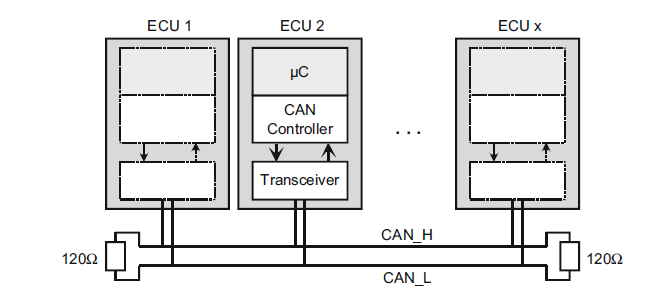
\includegraphics[width=0.8\textwidth]{./2_2_3_CAN-Netzwerk}
	\caption{CAN-Netzwerk: Ein einzelner \acs{CAN}-Knoten besteht aus einem Mikrocontroller, einem \acs{CAN}-Controller und einem \acs{CAN}-Transceiver. Der Abschlusswiderstand unterdrückt	Busreflexionen \cite{Zimmermann.2014}.}
	\label{abb:CANNetzwerk}
\end{figure}

Die physikalische Signalübertragung in einem \acs{CAN}-Netzwerk basiert auf der Übertragung von Spannungsdifferenzen zwischen der \emph{\acs{CAN}-High}-Leitung (CANH) und der \emph{\acs{CAN}-Low}-Leitung (CANL). Wie in Tabelle \ref{tab:KlassifikationSerielleBussysteme} dargestellt, unterscheidet die \acs{ISO}-Norm zwischen dem \emph{Low-Speed-\acs{CAN}} (Class B) und dem \emph{High-Speed-\acs{CAN}} (Class C). Der Low-Speed-\acs{CAN} zeichnet sich durch seine auf 125\,kbit/s begrenzte Datenrate aus. Dadurch findet er häufig in Komfortsystemen wie Klimasteuergeräten Anwendung. Die Signale werden über nominelle Potentiale auf dem Bus übertragen. Beim High-Speed-\acs{CAN} hingegen werden differentielle Potentiale verwendet. Dieser besitzt eine maximale Datenrate von bis zu 1\,Mbit/s und eignet sich daher für zeitkritische Anwendungen wie Antriebs- und Fahrdynamikregelung. Die unterschiedlichen Signalpegel werden in Abbildung \ref{abb:CANSignalpegel} erläutert. Aufgrund der Busankopplung ermöglicht der Low-Speed-\acs{CAN} zusätzliche Mechanismen zur Fehlererkennung. Bei Ausfall einer Leitung bleibt er betriebsfähig und gilt daher gegenüber dem High-Speed-\acs{CAN} als fehlertoleranter \cite{Zimmermann.2014, VectorInformatikGmbH.}.

\begin{figure}[!htbp]
	\centering
	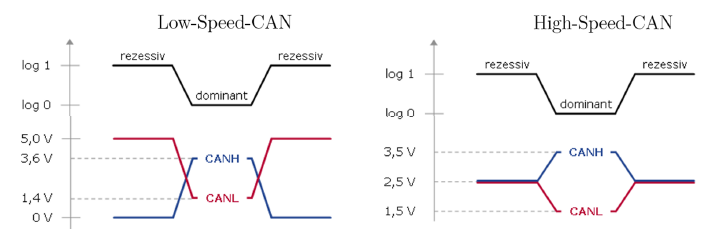
\includegraphics[width=\textwidth]{./2_2_3_Signalpegel-CAN}
	\caption{Signalpegel Low-Speed-\acs{CAN} (links) und High-Speed-\acs{CAN} (rechts) \cite{VectorInformatikGmbH.}.}
	\label{abb:CANSignalpegel}
\end{figure}

\subsection{CAN-Protokoll: Data Link Layer} \label{subsec:DataLinkLayer}
Der \emph{Data Link Layer} beschreibt das Zugriffsverfahren und den strukturellen Aufbau eines \acs{CAN}-\emph{Frames}. Unter einem Frame versteht man den gesamten Datenrahmen, der in einer einzelnen Botschaft über den \acs{CAN}-Bus übermittelt wird. Zwischen den Begriffen Frame, Botschaft und Nachricht wird nachfolgend keine Unterscheidung getroffen. Typischerweise gibt es mehrere Arten von CAN-Frames, die in verschiedene Kategorien unterteilt werden:

\begin{itemize}
	\item \emph{Data Frame} zur Übertragung von Nutzdaten.
	\item \emph{Remote Frame} zur Anforderung von Nutzdaten (also Data Frames) von beliebigen CAN-Knoten. Setzt sich bis auf das fehlende Data Field wie ein Data Frame zusammen.
	\item \emph{Error Frame} zur Signalisierung entdeckter Fehler während des Kommunikationsbetriebs. Mit dem Übertragen eines Error Frames geht der Abbruch der laufenden Botschaftsübertragung einher.
\end{itemize} 

Das Botschaftenformat eines Data Frames ist in Abbildung \ref{abb:CANDataFrame} dargestellt \cite{VectorInformatikGmbH.}. Die einzelnen Komponenten und deren Aufgaben werden nachstehend in der zugehörigen Tabelle \ref{tab:CAN-Data-Frame} näher erklärt.

\begin{figure}[!htbp]
	\centering
	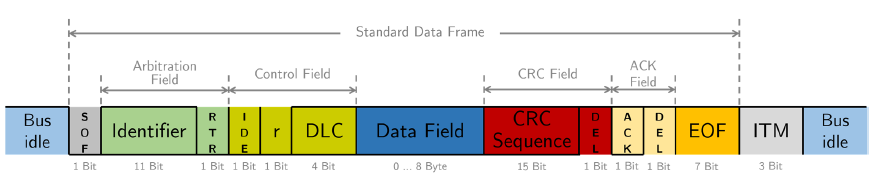
\includegraphics[width=\textwidth]{./2_2_4_CAN-Standard_Data_Frame}
	\caption{Aufbau des Standard \acs{CAN} Data-Frames \cite{VectorInformatikGmbH.}.}
	\label{abb:CANDataFrame}
\end{figure}

\begin{table}[!htb]
	\centering
	\caption{Funktionen der einzelnen Felder im Data-Frame \cite{Wallentowitz.2011, Zimmermann.2014}.}
	\footnotesize
	\renewcommand{\arraystretch}{1.3}
	\begin{tabular}{l | l l p{7.5cm}}
		\toprule
		Feld              & Name       & Länge       & Funktion                                                                                                                                                                                                          \\ \midrule
		kein Feld         & SOF        & 1 Bit       & Der dominante \emph{Start of Frame} signalisiert den Start eines Frames. Durch den Wechsel von einem rezessiven (Buspegel im Ruhezustand) auf ein dominantes Bit findet eine netzwerkweite Synchronisation statt. \\
		\midrule
		Arbitration Field & Identifier & 11 Bits     & Der Identifier dient der bitweisen Arbitrierung und beschreibt die logische Adressierung der Botschaft.                                                                                                           \\
		                  & RTR        & 1 Bit       & Der \emph{Remote Transmission Request} kennzeichnet	den Frametyp. Im Fall des Data Frames wird das Bit dominant übertragen.                                                                                       \\
		\midrule
		Control Field & IDE        & 1 Bit       & Die \emph{Identifier Extension} legt fest, ob der Identifier im Standard-Format (11 Bit) oder im Extended-Format (29 Bit) vorliegt.                                                                               \\
		                  & r          & 1 Bit       & Dieses Bit ist für künftige Erweiterungen reserviert.                                                                                                                                                             \\
		                  & DLC        & 4 Bits      & Der \emph{Data Length Code} übermittelt die Anzahl der nachfolgenden Nutzbytes.                                                                                                                                   \\
		\midrule
		Data Field        & Data Field & 0...64 Bits & Im Datenfeld werden bis zu acht Bytes an Nutzdaten übertragen. Es beinhaltet die zu übermittelnden Signalwerte und Nutzinformationen.                                                                             \\
		\midrule
		CRC-Field         & CRC        & 15 Bits     & Der \emph{Cyclic Redundancy Check} bildet eine Prüfsumme der Nutzdaten und dient der Fehlererkennung bei der Botschaftsübertragung.                                                                               \\
		                  & DEL        & 1 Bit       & Auf das CRC-Feld folgt ein rezessives \emph{Delimiter}-Bit.                                      \\
		\midrule
		ACK-Field         & ACK        & 1 Bit       & Der Sender einer Botschaft setzt das \emph{Acknowledgement}-Bit auf rezessiv, der Empfänger quittiert das korrekte Ergebnis des CRC-Feldes mit einem dominanten Bit.                                              \\
		                  & DEL        & 1 Bit       & Das ACK-Feld wird ebenfalls durch ein \emph{Delimiter}-Bit begrenzt.                                                                                                                                              \\
		\midrule
		kein Feld         & EOF        & 7 Bit       & Der \emph{End of Frame} markiert das Ende einer Botschaft mit sieben rezessiven Bits.                                                                                                                             \\ \bottomrule
	\end{tabular}
	
	\label{tab:CAN-Data-Frame}
\end{table}

Während der gesamten Laufzeit der Netzwerkverbindung senden die Busknoten ihre Botschaften nach dem \emph{Broadcast}-Verfahren unaufgefordert und ereignisgesteuert auf den Bus. Jeder Empfänger einer Botschaft entscheidet, ob der Inhalt relevant ist und er damit die Nachricht auswertet oder ignoriert. Diese \emph{Akzeptanzfilterung} findet auf Basis der inhaltsbasierten Adressierung eines Frames statt. Hierzu kennzeichnet der \emph{Identifier} \acs{ID} den spezifischen Inhalt einer Botschaft. Der Identifier ist in einem herkömmlichen \acs{CAN}-Protokoll 11 Bit lang. Somit lassen sich bis zu $2^{11} = 2.048$ Botschaften eindeutig unterscheiden. Aufgrund der stetig wachsenden Komplexität moderner Busarchitekturen besteht zudem die Möglichkeit, einen Identifier im Extended-Format aufzubauen. Der \acs{ID} umfasst dann 29 Bit, wodurch $2^{29} = 536.870.912$ unterschiedliche Botschaften differenziert werden können.\\
Durch den ereignisgesteuerten Kommunikationsaufbau kann es häufig vorkommen, dass mehrere Busteilnehmer eine Botschaftsübertragung zum gleichen Zeitpunkt beginnen möchten. Da eine Übertragung aber nicht unterbrochen werden kann und oftmals essenzielle sicherheitsrelevante Nachrichten unmittelbar mit vergleichsweise marginalen Botschaften versendet werden, ist es von hoher Bedeutung, sämtliche Botschaften mit Prioritäten zu versehen. Es wird das \emph{Carrier Sense Multiple Access with Collision Avoidance} \acs{CSMA/CA}-Verfahren angewendet. Durch eine \emph{bitweise Arbitrierung} wird dafür gesorgt, dass bei einer Kollision auf dem Bus die Botschaft mit der höchsten Priorität weiterhin übertragen wird. Die höchst priorisierte Botschaft weist immer den niedrigsten nominellen \acs{ID} auf. Durch den Vergleich der dominanten und rezessiven Buspegel ist jeder Knoten darüber informiert, welche Botschaft gerade auf dem Bus übertragen wird. Stellt ein Knoten der aktuell sendet fest, dass der Pegel auf dem Bus nicht seiner gesendeten Botschaft entspricht, stellt dieser umgehend den Sendevorgang ein. Die Echtzeitfähigkeit des Gesamtsystems wird somit nicht gefährdet und Botschaften mit hoher Priorität bleiben deterministisch. \\
Neben einer korrekten Zugriffsfolge sind besonders die Datensicherung und eine zuverlässige Fehlererkennung von großem Stellenwert. Hierzu kommen Mechanismen wie der \emph{Cyclic Redundancy Check} \acs{CRC}, \emph{Acknowledgement} \acs{ACK} oder \emph{Bitstuffing} zum Einsatz. In der \acs{CRC}-Sequenz wird aus dem Frame ein Polynom gebildet, welches durch Division mit einem Modulo-Operator eine Prüfsumme ergibt. Der Empfänger berechnet bei Erhalt einer Botschaft ebenfalls eine \acs{CRC}-Prüfsumme. Stimmen die erhaltenen und berechneten Sequenzen überein, war der strukturelle Aufbau der Botschaftsübertragung korrekt. Mindestens ein Empfänger bestätigt den positiven Erhalt, indem er das \acs{ACK}-Bit auf einen dominanten Pegel setzt. Liegt ein \acs{ACK}-Fehler vor, wurde also entweder vom Sender ein Fehler verursacht oder es befinden sich keine weiteren Teilnehmer am Bus.\\
Die Bitstuffing-Methodik dient der zeitlichen Nachsynchronisation während der Übertragungslaufzeit. Die Synchronisation der Busteilnehmer erfolgt eigentlich über den Flankenwechsel zwischen unterschiedlichen Bits. Liegen jedoch mehrere homogene Bits hintereinander vor, kann diese Synchronisation nicht stattfinden. Um eine korrekte Übertragung zu gewährleisten, fügt der Sender bis zum Ende der \acs{CRC}-Sequenz nach fünf homogenen Bits immer ein komplementäres Bit ein. Der Empfänger entfernt seinerseits diese Stuff-Bits, bevor das empfangene Datenpaket ausgewertet wird. Wird von einem Empfänger eine Folge von mehr als fünf homogenen Bits erkannt, liegt ein Bitstuffing-Fehler vor. Bei der Übertragung eines Data Frames mit 11 Bit Identifier kann der gesamte Botschaftsrahmen also um 29 Bit\footnote{im Worst Case bei acht Datenbytes} auf bis zu 132 Bit anwachsen. \\
Wurde einer der genannten Fehler erkannt, wird ein Fehlersignal gesetzt, welches aus sechs dominanten Bits besteht und damit bewusst gegen die Bitstuffing-Regel verstößt. In diesem Fall wird ein aktives \emph{Error Flag} in einem Error Frame von dem Knoten versendet, welcher den Sendefehler zuerst detektiert hat. Die beteiligten \acs{CAN}-Knoten stellen den Sendevorgang umgehend ein. Wird ein Fehler eines Knoten mehrfach detektiert, kann diesem das Senden verweigert werden. Zur Sicherstellung der systemweiten Datenkonsistenz und zur Reduzierung der Busauslastung kann ein fehlerhafter Knoten vollständig von der Buskommunikation ausgeschlossen werden \cite{Wallentowitz.2011, Zimmermann.2014, VectorInformatikGmbH.}.